%%%%%%%%%%%%%%%%%%%%%%%%%%%%%%%%%%%%%%%%%
% Beamer Presentation
% LaTeX Template
% Version 1.0 (10/11/12)
%
% This template has been downloaded from:
% http://www.LaTeXTemplates.com
%
% License:
% CC BY-NC-SA 3.0 (http://creativecommons.org/licenses/by-nc-sa/3.0/)
%
%%%%%%%%%%%%%%%%%%%%%%%%%%%%%%%%%%%%%%%%%

%----------------------------------------------------------------------------------------
%	PACKAGES AND THEMES
%----------------------------------------------------------------------------------------

\documentclass{beamer}

\mode<presentation> {

% The Beamer class comes with a number of default slide themes
% which change the colors and layouts of slides. Below this is a list
% of all the themes, uncomment each in turn to see what they look like.

%\usetheme{default}
%\usetheme{AnnArbor}
%\usetheme{Antibes}
%\usetheme{Bergen}
%\usetheme{Berkeley}
\usetheme{Berlin}
%\usetheme{Boadilla}
%\usetheme{CambridgeUS}
%\usetheme{Copenhagen}
%\usetheme{Darmstadt}
%\usetheme{Dresden}
%\usetheme{Frankfurt}
%\usetheme{Goettingen}
%\usetheme{Hannover}
%\usetheme{Ilmenau}
%\usetheme{JuanLesPins}
%\usetheme{Luebeck}
%\usetheme{Madrid}
%\usetheme{Malmoe}
%\usetheme{Marburg}
%\usetheme{Montpellier}
%\usetheme{PaloAlto}
%\usetheme{Pittsburgh}
%\usetheme{Rochester}
%\usetheme{Singapore}
%\usetheme{Szeged}
%\usetheme{Warsaw}

% As well as themes, the Beamer class has a number of color themes
% for any slide theme. Uncomment each of these in turn to see how it
% changes the colors of your current slide theme.

%\usecolortheme{albatross}
%\usecolortheme{beaver}
%\usecolortheme{beetle}
%\usecolortheme{crane}
%\usecolortheme{dolphin}
%\usecolortheme{dove}
%\usecolortheme{fly}
%\usecolortheme{lily}
%\usecolortheme{orchid}
%\usecolortheme{rose}
%\usecolortheme{seagull}
%\usecolortheme{seahorse}
%\usecolortheme{whale}
%\usecolortheme{wolverine}

%\setbeamertemplate{footline} % To remove the footer line in all slides uncomment this line
%\setbeamertemplate{footline}[page number] % To replace the footer line in all slides with a simple slide count uncomment this line

%\setbeamertemplate{navigation symbols}{} % To remove the navigation symbols from the bottom of all slides uncomment this line
}

\usepackage{graphicx} % Allows including images
\usepackage{booktabs} % Allows the use of \toprule, \midrule and \bottomrule in tables
%\usepackage[brazilian]{babel}
\usepackage[utf8]{inputenc}
\usepackage{listings}
\usepackage{amsmath}
\usepackage{amsfonts}
\usepackage{pdfpages}
\usepackage{textpos}

\graphicspath{ {img/} }

%----------------------------------------------------------------------------------------
%	TITLE PAGE
%----------------------------------------------------------------------------------------

\title[Generating Acrostics via Paraphrasing and Heuristic Search]{Generating Acrostics via Paraphrasing and Heuristic Search} % The short title appears at the bottom of every slide, the full title is only on the title page

\author[Bruno, Fernando, Jürgen, William]{Bruno Soares Fillmann\\
Fernando Bombardelli da Silva\\
Jürgen Bauer\\
William Bombardelli da Silva
} % Your name
\institute[TU Berlin] % Your institution as it will appear on the bottom of every slide, may be shorthand to save space
{
Technische Universität Berlin \\ % Your institution for the title page
Datenbanksysteme und Informationsmanagement \\
DBPRO – Database Projects (WS 2014/2015) \\
\medskip
%\textit{fbdasilva@inf.ufrgs.br} % Your email address
}
\date{01.12.2014} % Date, can be changed to a custom date

\begin{document}

\begin{frame}
\titlepage % Print the title page as the first slide
\end{frame}

\begin{frame}
\frametitle{Organisation} % Table of contents slide, comment this block out to remove it
\tableofcontents % Throughout your presentation, if you choose to use \section{} and \subsection{} commands, these will automatically be printed on this slide as an overview of your presentation
\end{frame}

%----------------------------------------------------------------------------------------
%	PRESENTATION SLIDES
%----------------------------------------------------------------------------------------

%------------------------------------------------
\section{Overview} % Sections can be created in order to organize your presentation into discrete blocks, all sections and subsections are automatically printed in the table of contents as an overview of the talk
%------------------------------------------------

%\subsection{Subsection Example} % A subsection can be created just before a set of slides with a common theme to further break down your presentation into chunks

\begin{frame}
\frametitle{Overview}
\begin{itemize}
\item \textbf{Entrada:} Um grafo virtual e um grafo do substrato físico
\item \textbf{Problema de Localização:} Encontrar um mapeamento \emph{válido} dos vértices do grafo virtual para os vértices do grafo físico, assim como das arestas do virtual para caminhos no físico
\item \textbf{Problema de Otimização:} Minimizar a banda total utilizada pelo mapeamento
\end{itemize}
\end{frame}

\begin{frame}
\frametitle{Classes Diagram}
\end{frame}

\begin{frame}
\frametitle{Activity Diagram and Search Strategy}
\end{frame}

%------------------------------------------------
\section{Implemented Operations}
%------------------------------------------------

\begin{frame}
\frametitle{Line Break}


\begin{itemize}
\item Constraints on line length $l_{min}=50$ and $l_{max}=70.$



\item Two cases: 



\begin{itemize}
\item After a word when line length falls in the\\
 $[l_{min},l_{max}]$-window.
\item After a full stop. (i.e., paragraph break)
\end{itemize}


\item Succeeding line break, lines have to be aligned.

\item A greedy word wrap algorithm is applied. 

\item Avoid words of length $>20$ in the start text.
\end{itemize}




\end{frame}



\begin{frame}
\frametitle{Line Break}

%\begin{textblock}{200}(0,0)
%\leavevmode
%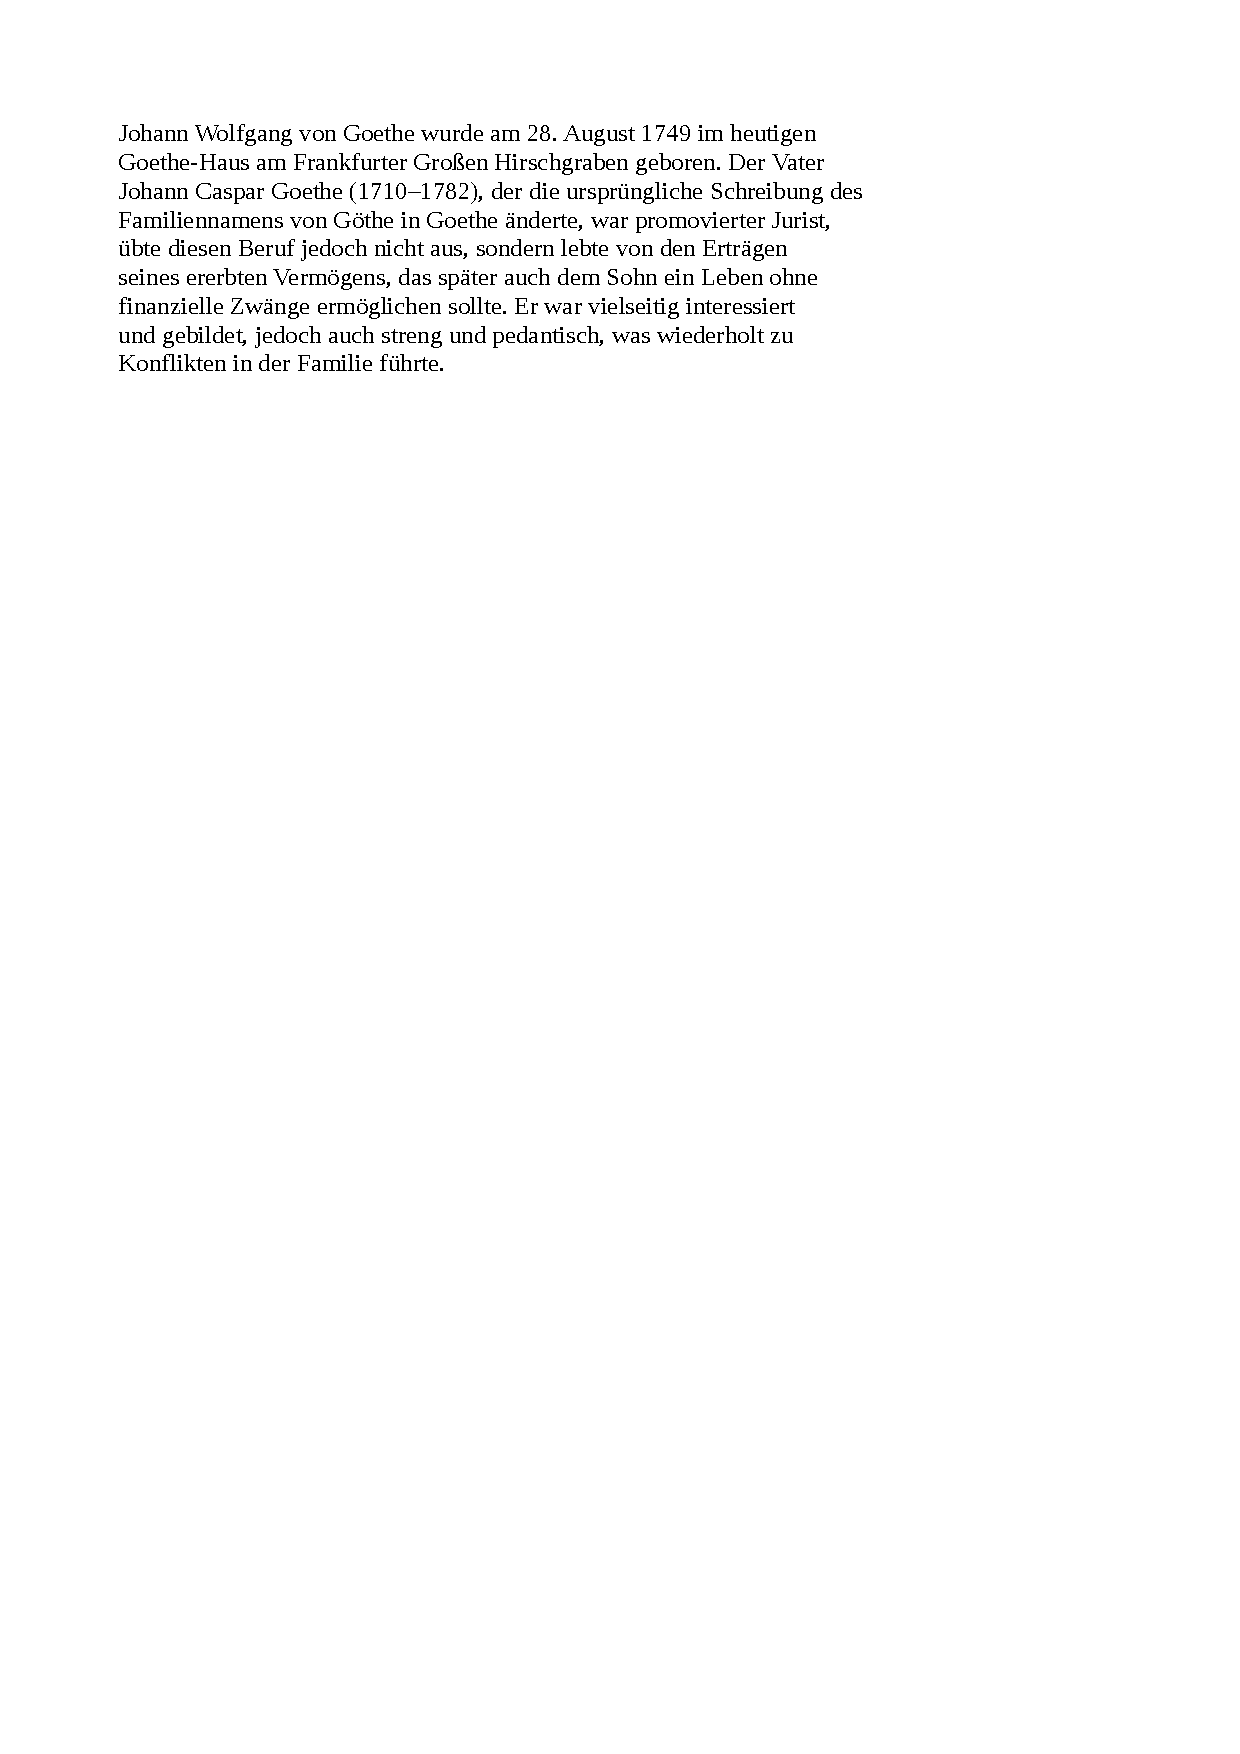
\includegraphics[scale=0.5]{Goethe.pdf}

%\put(0,50){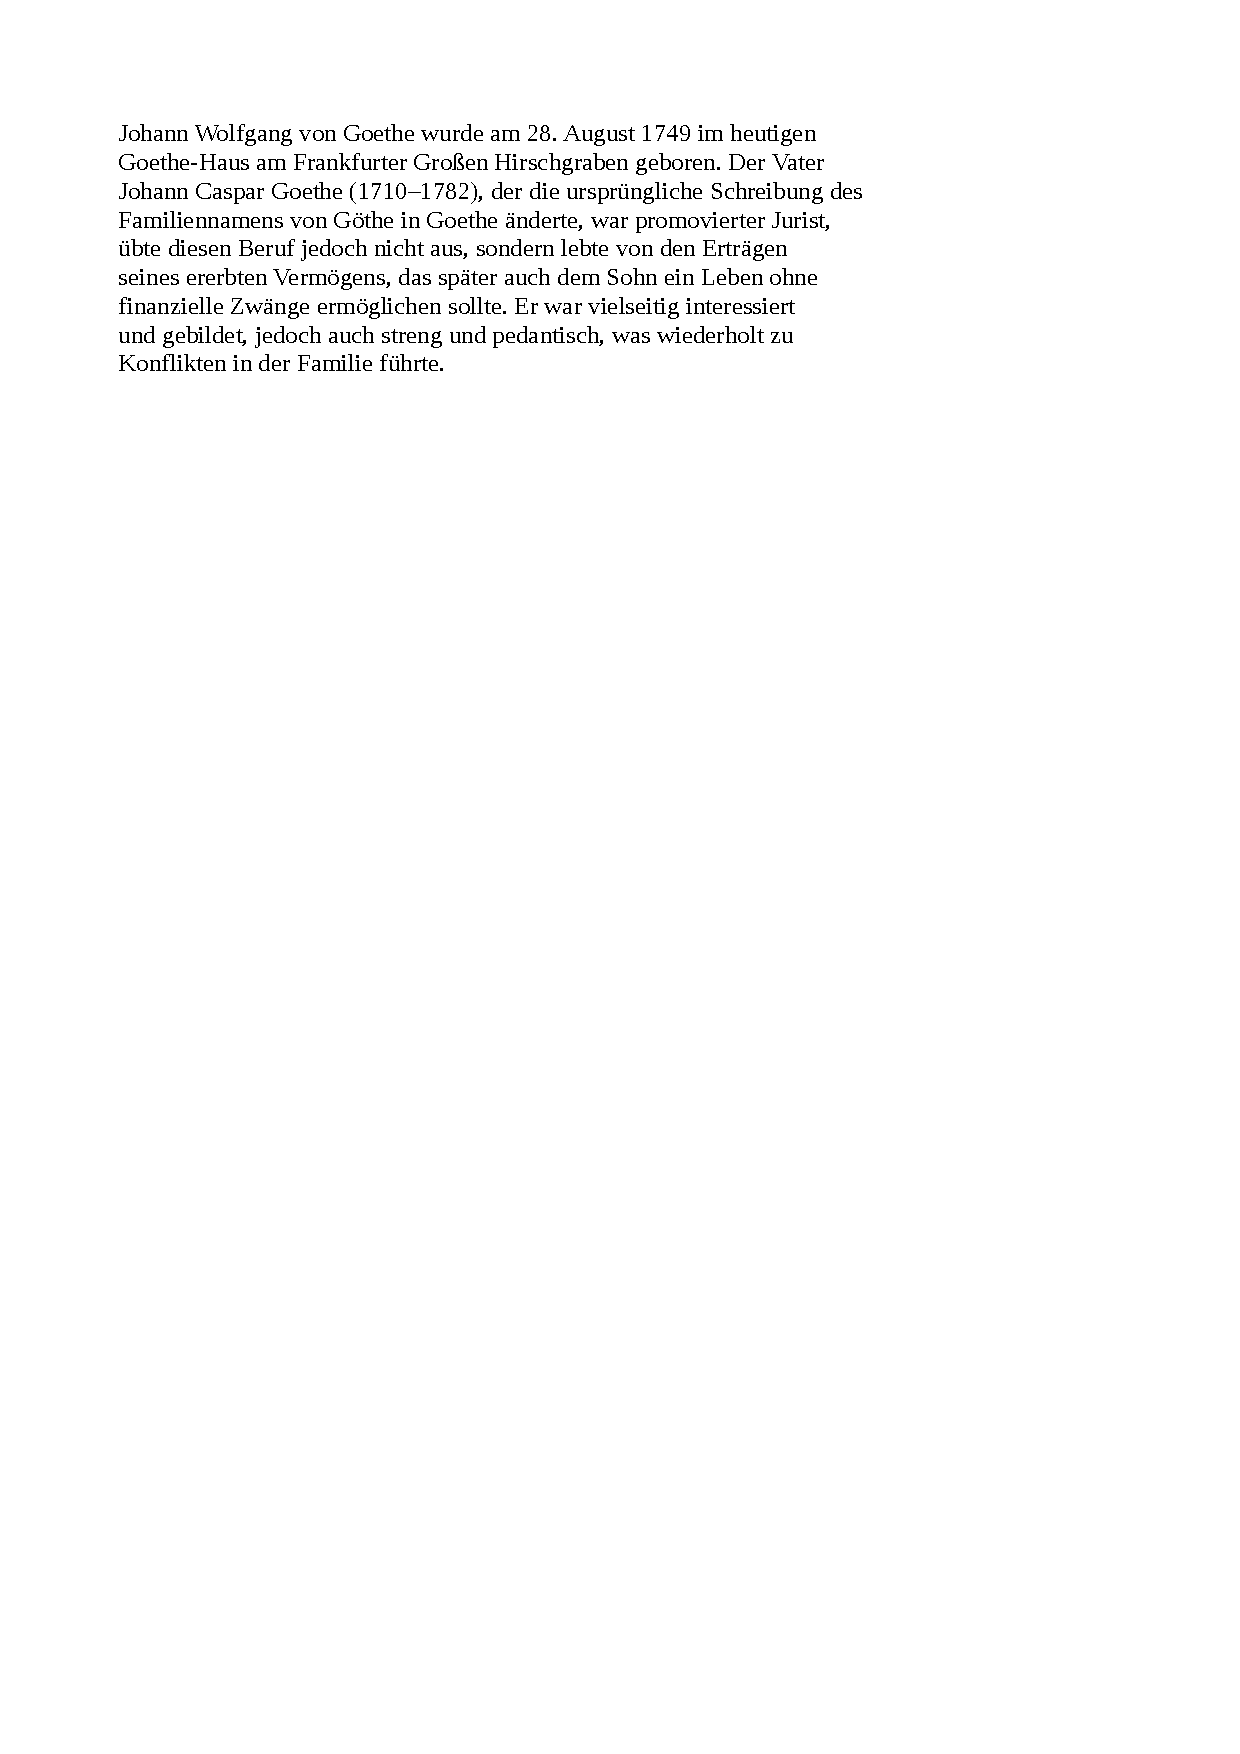
\includegraphics[scale=0.5]{Goethe.pdf}}
%\end{textblock}

\begin{itemize}
\item \textbf{Example:}
\item 18 linebreaks,
\item No full stop after 28!
\item Third often applied operator on a solution path
\item Fastest operator
%\item Hier steht ein längerer Text mit Foto
%\end{itemize}

\end{itemize}

\begin{picture}(300,400)
\put(-10,-165){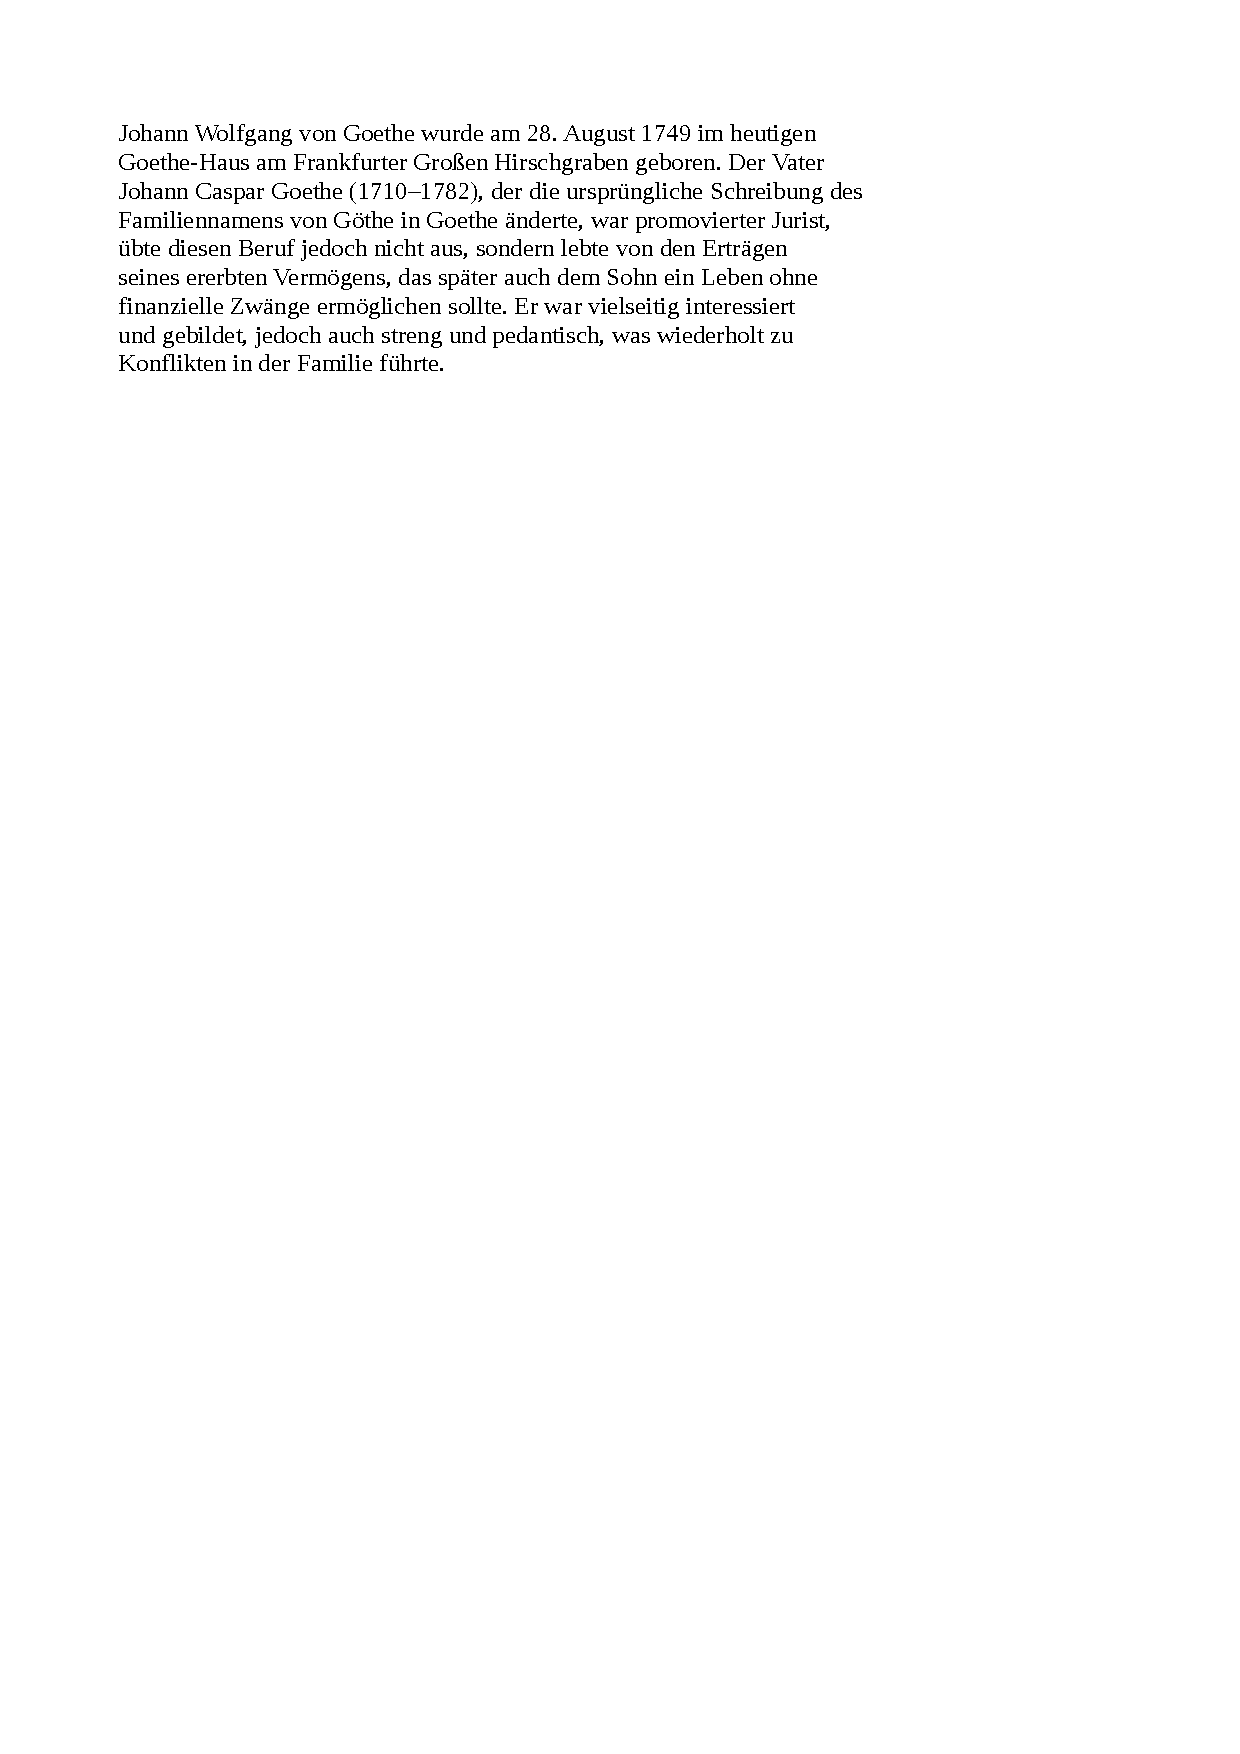
\includegraphics[scale=0.7]{Goethe.pdf}}
\end{picture}





%\begin{picture}(220,450)
%\put(40,80){ 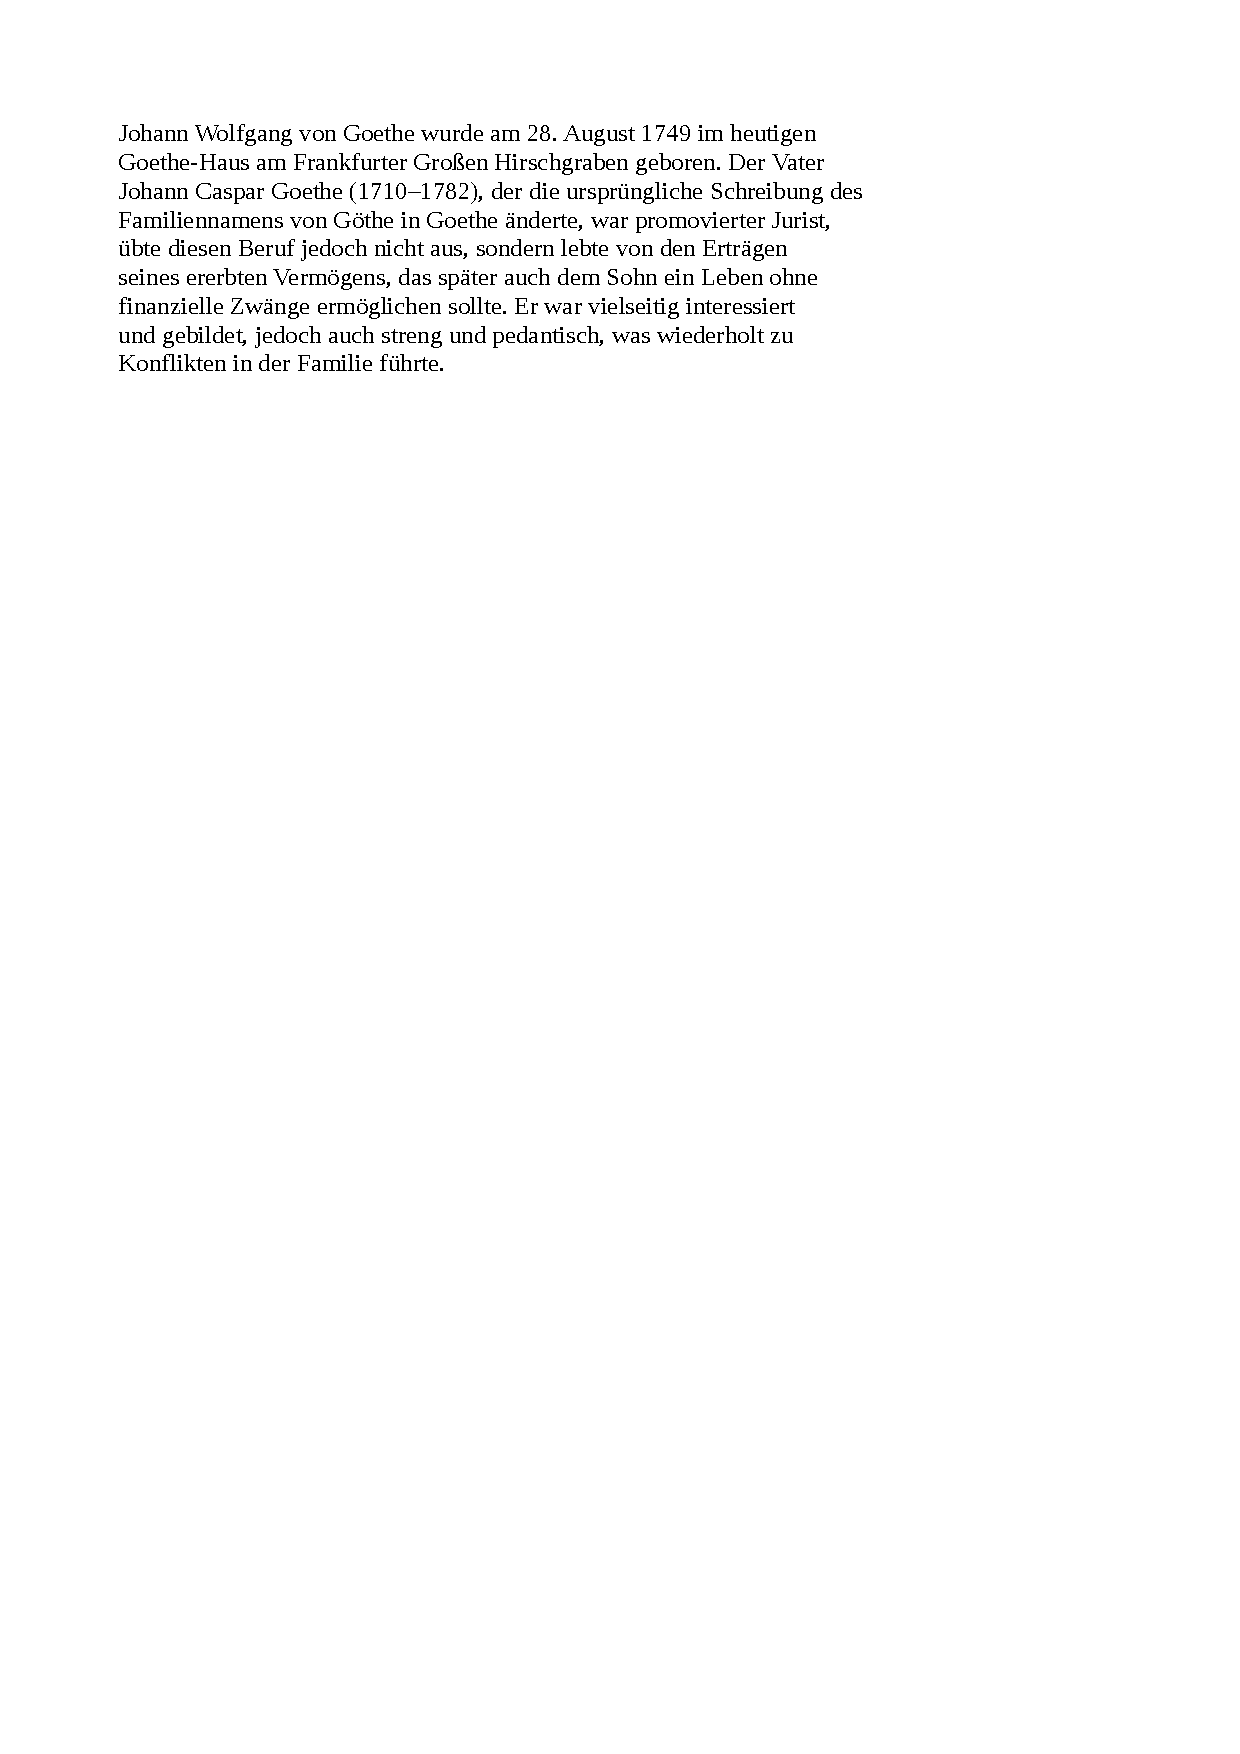
\includegraphics[height=15\textheight]{Goethe.pdf} }
%\end{picture}



\end{frame}











\begin{frame}
\frametitle{Wrong Hyphenation}

 
\end{frame}

\begin{frame}
\frametitle{Ensure Constraints}
\end{frame}

\begin{frame}
\frametitle{Word Insertion}
\end{frame}

%------------------------------------------------
\section{First Results}
%------------------------------------------------

\begin{frame}
\frametitle{First Results}
\begin{itemize}
\item \textbf{\emph{Solver} GNU GLPK:} Execução por um longo período sem produção de resultados finais
\end{itemize}
\begin{table}[H]
\centering
\begin{tabular}{|l | r |}
	\hline
	\textbf{Parâmetro} & \textbf{Valor} \\ \hline
	Iterações externas		& 1000	\\ \hline
	Iterações internas		& 300	\\ \hline
	Mínimo de iterações com sucesso	& 10 	\\ \hline
	Coeficiente de resfriamento		& 0.99	\\ \hline
\end{tabular}
\caption{Parâmetros do Algoritmo}
\label{tab:Parametros}
\end{table}
\end{frame}

%------------------------------------------------
\section{Next Steps}
%------------------------------------------------

\begin{frame}
\frametitle{Next Steps}
\begin{itemize}
\item Mapeamento de redes virtuais é complexo até mesmo para localização de solução inicial
\item Importância do algoritmo de vizinhança para uma boa convergência do método
\item \emph{Solvers} genéricos não são viáveis na prática
\item Decisões na fase de projeto do algoritmo são cruciais para o resultado com a meta-heurística
\end{itemize}
\end{frame}

%------------------------------------------------

\begin{frame}
\Huge{\centerline{Questions?}}
\end{frame}

%----------------------------------------------------------------------------------------

\end{document}